\paragraph{QuizziPedia::Front-End::Services::QuestionsService}
\begin{figure}[ht]
	\centering
	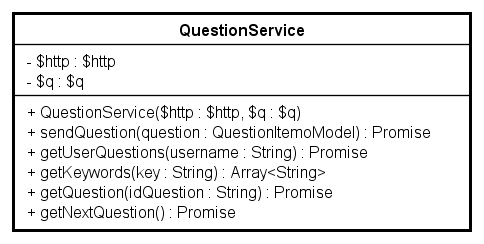
\includegraphics[scale=0.60]{UML/Classi/Front-End/QuizziPedia_Front-end_Services_QuestionService.png}
	\caption{QuizziPedia::Front-End::Services::QuestionService}
\end{figure}\FloatBarrier
\begin{itemize}
	\item \textbf{Descrizione}: questa classe permette di ottenere domande esistenti e salvare nuove domande;
	\item \textbf{Utilizzo}: utilizzata per richiedere domande presenti nel database. Offre inoltre delle funzionalità per inserire nuove domande;
	\item \textbf{Relazione con altre classi:}
	\begin{itemize}
		\item \textit{IN} \texttt{QuestionItemModel}: rappresenta una domanda. Contiene tutte le informazioni necessarie alla
		presentazione del contenuto della domanda; 
		\item \textit{IN} \texttt{TrueFalseQuestionsController}: questa classe permette di gestire la creazione e la modifica di una domanda vero/falso;
		\item \textit{IN} \texttt{MultiplyQuestionsController}: questa classe permette di gestire la creazione e la modifica di una domanda a risposta multipla; 
		\item \textit{IN} \texttt{ConnectionQuestionsController}: questa classe permette di gestire la creazione e la modifica di una domanda a collegamento;
		\item \textit{IN} \texttt{ImagesSortingQuestionsController}: questa classe permette di gestire la creazione e la modifica di una domanda a ordinamento immagini;
		\item \textit{IN} \texttt{StringsSortingQuestionsController}: questa classe permette di gestire la creazione e la modifica di una domanda a ordinamento di stringhe;
		\item \textit{IN} \texttt{FillingQuestionsController}: questa classe permette di gestire la creazione e la modifica di una domanda a riempimento di spazi; 
		\item \textit{IN} \texttt{ClickableAreaQuestionsController}: questa classe permette di gestire la creazione e la modifica di una domanda ad area cliccabile;
		\item \textit{IN} \texttt{EditorQMLController}: questa classe permette di gestire la creazione e la modifica di domande create tramite editor QML;
		\item \textit{IN} \texttt{QuestionsManagementController}: questa classe permette di gestire e di ottenere le domande create dall'utente;
		\item \textit{IN} \texttt{TopicKeywordsController}: questa classe permette di gestire il recupero delle parole chiave di un questionario;
		\item \textit{IN} \texttt{QuestionnaireQuestionsManagementController}: questa classe permette di gestire il recupero delle domande per il questionario;
		\item \textit{IN} \texttt{QuestionsController}: questa classe permette di gestire il recupero delle domande per poterle stampare nella modalità allenamento;
		\item \textit{IN} \texttt{QuestionsItemModel}: rappresenta una domanda. Contiene tutte le informazioni necessarie alla presentazione del contenuto della domanda.
		
	\end{itemize}
	\item \textbf{Attributi:}
	\begin{itemize}
		\item \texttt{-} \texttt{\$http: \$http} \\ Campo dati che contiene un riferimento al servizio \$http che permette la comunicazione con il protocollo \textit{HTTP\ped{G}};
		\item \texttt{-} \texttt{\$q: \$q} \\ Campo dati che contiene un riferimento a \$q, un servizio offerto da \textit{AngularJS\ped{G}} per la gestione, tramite \textit{Promise\ped{G}}, di chiamate asincrone.
	\end{itemize}
	\item \textbf{Metodi:}
	\begin{itemize}
		\item \texttt{+} \texttt{QuestionService(\$http: \$http, \$q: \$q)} \\ Metodo costruttore della classe. \\
		\textbf{Parametri}:
		\begin{itemize}
			\item \texttt{-} \texttt{\$http: \$http} \\ Campo dati che contiene un riferimento al servizio \$http che permette la comunicazione con il protocollo \textit{HTTP\ped{G}};
			\item \texttt{-} \texttt{\$q: \$q} \\ Campo dati che contiene un riferimento a \$q, un servizio offerto da \textit{AngularJS\ped{G}} per la gestione, tramite \textit{Promise\ped{G}}, di chiamate asincrone.
		\end{itemize}
		\item \texttt{+} \texttt{sendQuestion(question: QuestionItemModel): Promise} \\Metodo che serve per mandare una domanda al back-end in modo che venga salvata; In caso la \textit{Promise\ped{G}} venga rifiutata, verrà restituito al controller un oggetto \texttt{ErrorModelInfo} contenente tutti i dettagli dell'errore. In caso la \textit{Promise\ped{G}} venga accettata, verrà restituito al chiamante del metodo il risultato della chiamata.\\
		\textbf{Parametri}: 
		\begin{itemize}
			\item \texttt{question: QuestionItemModel} \\ Identifica tutti i dettagli di una domanda.
		\end{itemize}
		\item \texttt{+} \texttt{getUserQuestions(username: String): Promise} \\Metodo che ritorna tutte le domande create dall'utente. Il metodo ritorna una \textit{Promise\ped{G}}. In caso la \textit{Promise\ped{G}} venga rifiutata, verrà restituito al \texttt{QuestionsManagementController} un oggetto \texttt{ErrorModelInfo} contenente tutti i dettagli dell'errore. In caso la \textit{Promise\ped{G}} venga accettata, verrà restituito al chiamante del metodo il risultato della chiamata.\\
		\textbf{Parametri}:
		\begin{itemize}
			\item \texttt{username: String} \\ Parametro che indica l'utente del quale andranno caricate tutte le domande da lui create.
		\end{itemize}
		\item \texttt{+} \texttt{getKeywords(key: String): String[]}\\ Metodo che permette di ottenere le keywords a partire da una stringa passata.\\
		\textbf{Parametri}:
		\begin{itemize}
			\item \texttt{key: String} \\ Parametro che identifica la stringa con la quale cercare le keywords.
		\end{itemize}
		\item \texttt{+} \texttt{getQuestion(idQuestion: String): Promise} \\ Metodo che ritorna la domanda associata all'id passato come parametro. Il metodo ritorna una \textit{Promise\ped{G}}. In caso la \textit{Promise\ped{G}} venga rifiutata, verrà restituito al \texttt{QuestionsManagementController} un oggetto \texttt{ErrorModelInfo} contenente tutti i dettagli dell'errore. In caso la \textit{Promise\ped{G}} venga accettata, verrà restituito al chiamante del metodo il risultato della chiamata.\\
		\textbf{Parametri}:
		\begin{itemize}
			\item \item \texttt{idQuestion: String} \\ Parametro che indica l'id della domanda da recuperare e restituire.
		\end{itemize}
		\item \texttt{+} \texttt{getNextQuestion(): Promise} \\ Metodo che ritorna la domanda successiva nella modalità allenamento. Il metodo ritorna una \textit{Promise\ped{G}}. In caso la \textit{Promise\ped{G}} venga rifiutata, verrà restituito al \texttt{QuestionsController} un oggetto \texttt{ErrorModelInfo} contenente tutti i dettagli dell'errore. In caso la \textit{Promise\ped{G}} venga accettata, verrà restituito al chiamante del metodo il risultato della chiamata.
	\end{itemize}
\end{itemize}